\documentclass[13pt, a4paper]{elsarticle}
\usepackage{amssymb, amsthm, amsmath}
\usepackage{siunitx}
\usepackage{graphicx}
\usepackage{setspace}
\usepackage{float}
\usepackage{caption}
\usepackage{subcaption}
\usepackage{mathtools, cuted}
\usepackage{titletoc}
\usepackage[left=3.5cm,right=2.0cm,top=3.5cm,bottom=3.0cm]{geometry}
\usepackage[utf8]{vietnam}
%\usepackage{times}
\biboptions{numbers,sort&compress}
\usepackage[breaklinks,colorlinks=true,citecolor={black}, linkcolor= {black}, urlcolor ={black}]{hyperref}

% ====================================================================================
\begin{document}
\onehalfspacing
\section{Giới thiệu tổng quan} 
Độ hấp thụ quang của graphene đơn lớp trong miền ánh sáng khả kiến chỉ vào khoảng $A=\pi \alpha\approx \SI{2.3}{\percent}$ với $\alpha$ là hằng số cấu trúc tinh tế \cite{R.R.NairFSC}. Độ hấp thụ ánh sáng $\SI{2.3}{\percent}$ cũng được xem là khá lớn đối với một bản vật liệu mỏng nhưng vẫn chưa đủ cho các ứng dụng thực tế như cảm biến quang hay các thiết bị nhiệt định xứ (local heating devices) như ý tưởng của Nulli và các cộng sự \cite{NulliAPL18}.\\
Năm 2018, tính toán lý thuyết của nhóm tác giả tại Đại học Tohoku đã chứng minh rằng, bằng cách đặt graphene đơn lớp ở tâm cấu trúc đa lớp đối xứng được tạo ra bởi hai lớp điện môi xen kẽ nhau theo sơ đồ: $ABABAB\textbf{G}BABABA$, trong đó $A, B, G$ lần lượt là các lớp điện môi và lớp graphene, thì độ hấp thụ quang học trong lớp graphene có thể tăng lên đến $\SI{50}{\percent}$  khi thay đổi số lớp hoặc chiết suất các lớp điện môi thích hợp. Độ hấp thụ ánh sáng trong graphene ở tâm cấu trúc có thể được tăng cường với tần số ánh sáng tới tùy ý miễn là độ dày mỗi lớp điện môi tương ứng với một phần tư bước sóng \cite{NulliAPL18}. Nhóm tác giả cũng chỉ ra rằng, để đạt được độ hấp thụ mạnh phải cần hai lớp vật liệu có tỉ số chiết suất $\gamma=n_A/n_B$ đủ lớn, hoặc nếu việc tìm kiếm vật liệu với $\gamma$ lớn là khó khăn thì chúng ta phải sử dụng nhiều lớp điện môi trong cấu trúc. Ví dụ, để đạt được độ hấp thụ $\SI{50}{\percent}$ thì $\gamma=3.05$ với $s=2$, hoặc $\gamma=1.56$ và $s=5$ trong đó $s$ là số cặp vật liệu $AB$ được sử dụng \cite{NulliAPL18}. Như vậy, việc tìm được hai loại vật liệu có tỉ số chiết suất đủ lớn hay chế tạo nhiều lớp vật liệu có kích thước vi mô đồng nhất (tương ứng một phần tư bước sóng ánh sáng tới) là một vấn đề phức tạp trong thực nghiệm.
\section{Mục đích nghiên cứu}
Chúng tôi mong muốn kiểm tra về mặt lý thuyết khả năng tăng cường độ hấp thụ của graphene đơn lớp thông qua khảo sát điện trường ở bề mặt của graphene được đặt trong vi hốc cộng hưởng tạo bởi hai lớp vàng mỏng như Hình \ref{fig:1}. 
\begin{figure}[h]
	\centering
	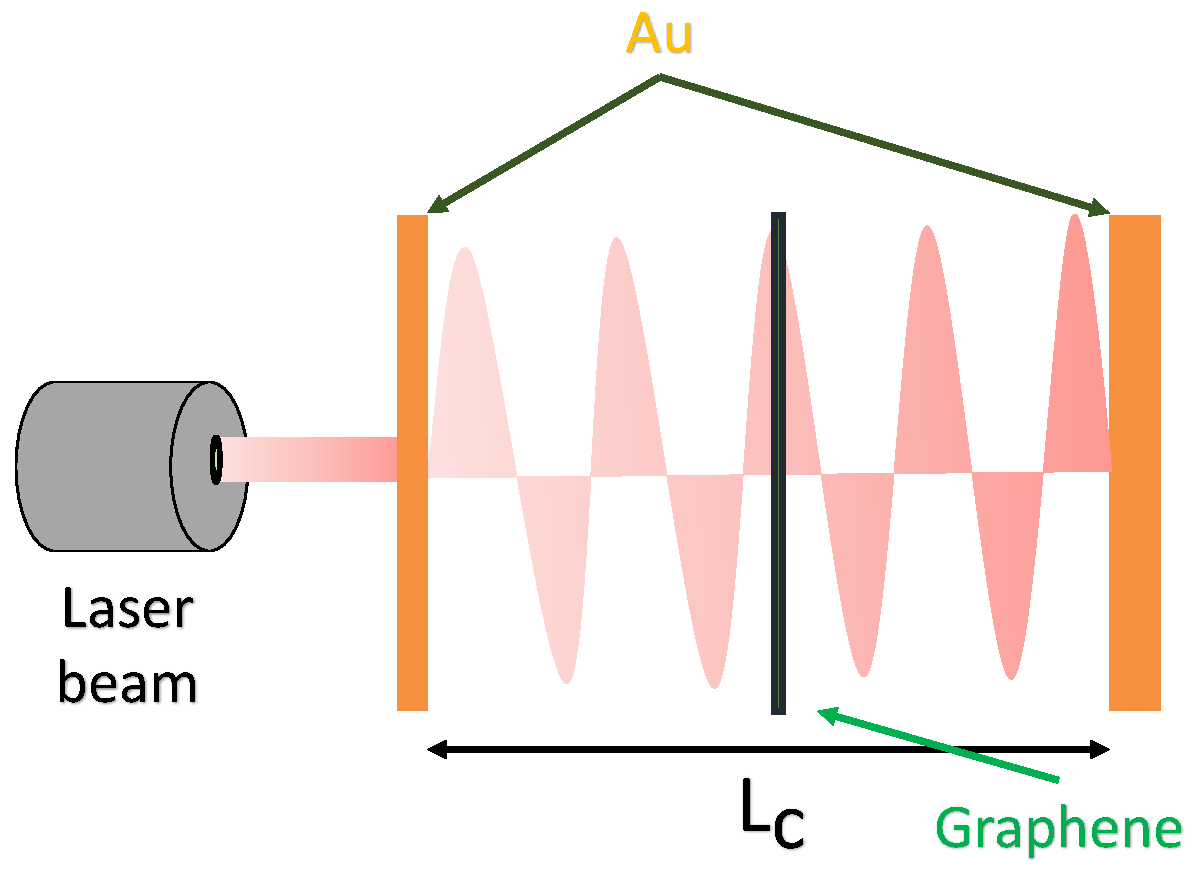
\includegraphics[width=0.6\linewidth]{figs/fig1model.pdf}
	\caption{Mô hình vi hốc cộng hưởng tạo bởi hai lớp vàng mỏng, lớp graphene được đặt giữa vi hốc.}
	\label{fig:1}
\end{figure}
\section{Đối tượng nghiên cứu}
Độ hấp thụ quang học của lớp graphene được đặt trong vi hốc cộng hưởng khi được chiếu bằng nguồn laser bước sóng $\lambda=\SI{632.82}{\nano\meter}$.
\section{Phương pháp nghiên cứu}
\begin{itemize}
	\item Maxwell stress tensor.
	\item Phương pháp ma trận truyền (Transfer matrix method) được đề xuất bởi \cite{ZhanTMM}.
\end{itemize}
\section{Nội dung và phạm vi của vấn đề sẽ đi sâu nghiên cứu}
\begin{itemize}
	\item Tìm hiểu tính chất quang học của graphene, Maxwell stress tensor, phương pháp ma trận truyền cho bài toán quang học, độ hấp thụ quang của vật liệu, \dots
	\item Sử dụng ngôn ngữ lập trình Python trong việc tính toán khảo sát độ hấp thụ quang của graphene trong vi hốc cộng hưởng.
	\item Khảo sát sự ảnh hưởng của vi hốc cộng hưởng đối với độ hấp thụ quang học của graphene: góc tới, bề dày 2 lớp vàng, khoảng cách giữa hai lớp vàng.
\end{itemize}
\section{Thời gian thực hiện}
\begin{tabular}{|>{\centering\arraybackslash}m{6cm}|>{\centering\arraybackslash}m{9cm}|}
	\hline
	\textbf{Thời gian} & \textbf{Nội dung}\\
	\hline
	Tháng 10/2023 - tháng 01/2024 & Nghiên cứu cơ sở lý thuyết của đề tài, tìm hiểu các công cụ hỗ trợ: Python.\\
	\hline
	Tháng 01/2024 - tháng 07/2024 & Thực hiện đề tài luận văn.\\
	\hline
	Tháng 07/2024 - tháng 09/2024 & Chỉnh sửa nội dung báo cáo, chuẩn bị bảo vệ luận văn tốt nghiệp.\\
	\hline
	Tháng 10/2023 & Bảo vệ luận văn tốt nghiệp.\\
	\hline
\end{tabular}
\bibliographystyle{elsarticle-num}
\bibliography{SangRef_2023}
\end{document}

%\endinput
